\section{Laplace Transformation}
\subsection{Definition}
Annahme: Funktionen $f(t)$ sind so, dass
\begin{equation*}
    f(t)=0, \hspace{1em} t\leq0
\end{equation*}
\begin{center}
    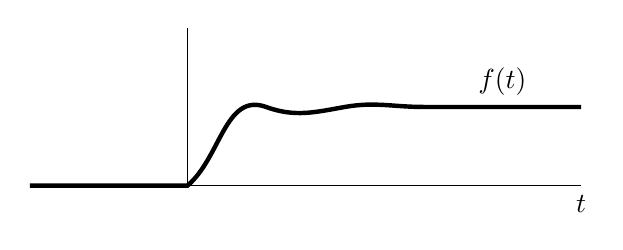
\begin{tikzpicture}
        \draw (0,2) -- (0,0) -- (5,0) node[below] {$t$};
        \draw[ultra thick] (-2,0) -- (0,0) 
            to[out=40,in=160] (1,1) 
            to[out=-20,in=190] (2,1)
            to[out=10,in=180] (3,1)
            -- (5,1) 
            node[pos=0.5,above] {$f(t)$};
    \end{tikzpicture}
\end{center}
\definition{Definition}{Laplace Transformation von $f(t)$}
\begin{equation*}
    \boxed{
        F(s) = \int_0^\infty f(t) e^{-st}\text{d}t
    }
\end{equation*}

Schreibweise:
\begin{eqnarr}
    F(s) &=&  \L (f(t)) \\
    F\tikzmark{a}(s) &\multimapdotbothA& f\tikzmark{b}(t)
\end{eqnarr}
\begin{center}
    \begin{tikzpicture}[overlay,remember picture]
        \node at (-2,0) (ta) {Bildfunktion};
        \node at (2,0) (tb) {Originalfunktion};
        \draw[->,thick] (ta) to (a);
        \draw[->,thick] (tb) to (b);
    \end{tikzpicture}
\end{center}

